\subsection{Hardware and Software}

The setup for the experiment used a 1st generation 84" Microsoft Surface Hub. On
the display, we full-screened a Chrome window that displayed the test. The screen
had a resolution of 3840px by 2160px. Particiapnts stood 3m from the center
of the screen. The server powering the application which
both the Surface Hub and user's cellphones connected had an average ping to both
of around 110ms. For both the Surface Hub and cellphones, the application was
navigated to within the web browser, where interactions were recorded in
real time, and communication handled via a duplex WebSocket connection on all
clients. For the experiment, participants utilized their own phones with no
additional software or browsers installed that they had to use, helping to ensure
generalizability of our approach.

For the experiment, we utilized a striped down, modified version of the MUIFOLD
interface, with some re-arrangement of buttons, and the ability for users to 
control both the mode of pointing, sensitivity, and the coefficient applied to 
smoothing, as shown in Figure~\ref{fig:experiment_ui}.
For the two modes of pointing, ``coarse'' would at the default 
sensitivity move the cursor 55 pixels per degree change while ``fine'' would
move the cursor 20 pixels. These factors were derived via a fixed expected
angle of interaction by the user from the set distance away from the screen,
adjusted slightly downwards as users were not really going towards the edge
of the screen. The ``Start Pointing'' / ``Stop Pointing'' and 
``Click'' buttons operated the same as in the main MUIFOLD interface. We wished
to see if users would want to modify their sensitivity settings so as to help
us adjust our initial settings based on pure laboratory conditions. The software,
similar to above, only considered changes in yaw and pitch for moving the
user's on-screen cursor.

\begin{figure}
\centering
  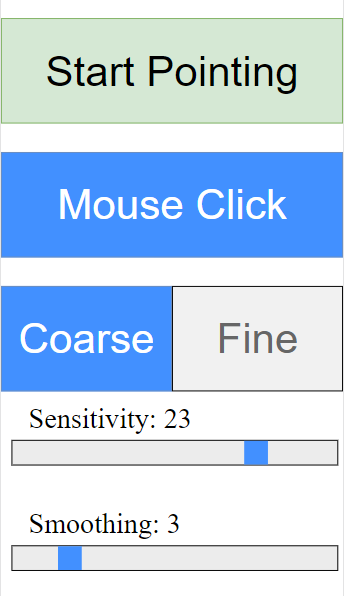
\includegraphics[width=0.4\columnwidth]{chapters/04_muifold/figures/experiment_ui.png}
  \caption{Cellphone UI as shown to users during the experiment.}
  \label{fig:experiment_ui}
\end{figure}